\section{Advanced Tasks: Diarization \& Emotion Recognition}

\begin{frame}{}
    \LARGE \textbf{Advanced Tasks: Diarization \& Emotion Recognition}
\end{frame}

\begin{frame}[allowframebreaks]{Speaker Diarization}
    \begin{itemize}
        \item \textbf{Goal:} Identify ``who spoke when'' in audio streams
        \item \textbf{Applications:}
            \begin{itemize}
                \item Meeting transcription
                \item Podcast analysis
                \item Call center monitoring
            \end{itemize}
        \item \textbf{Pipeline:}
            \begin{enumerate}
                \item \textbf{Voice activity detection (VAD):} separate speech from silence and noise
                \item \textbf{Segmentation:} cut the speech into windows, or detect speaker change points
                \item \textbf{Embedding:} map each segment to a speaker vector (x-vector, ECAPA-TDNN)
                \item \textbf{Clustering:} group segments by speaker from pairwise similarities
                \item \textbf{Resegmentation:} refine the boundaries and assign overlapping speech
            \end{enumerate}
    \end{itemize}
\framebreak
    VAD comes first for a reason: any speech it drops is lost for good, and any noise it admits gets assigned to some speaker. Its errors propagate through every later stage.
    \begin{center}
        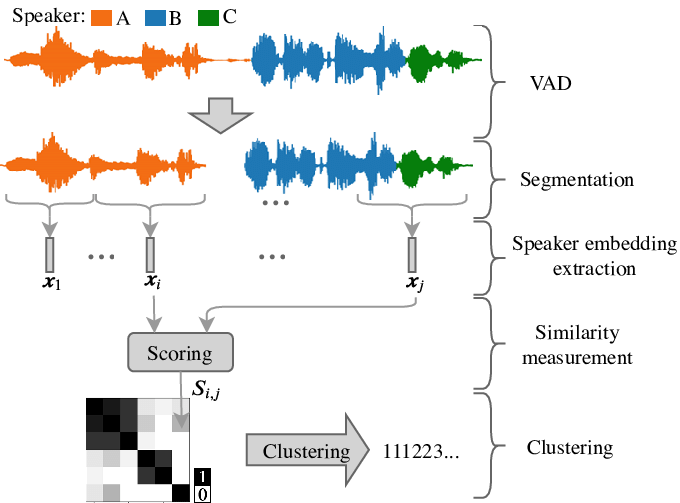
\includegraphics[width=\textwidth,height=0.66\textheight,keepaspectratio]{images/audio-nlp/diarization_pipeline.png}\\
        {\scriptsize Source: Q.~Lin, Y.~Hou and M.~Li, ``Self-Attentive Similarity Measurement Strategies in Speaker Diarization,'' Interspeech 2020, Fig.~1.}
    \end{center}
\end{frame}

\begin{frame}[allowframebreaks]{Speaker Diarization Tools}
    \begin{itemize}
        \item \textbf{Popular Tool:} \texttt{pyannote.audio} (Bredin et al., ICASSP 2020)
        \item \textbf{Features:}
            \begin{itemize}
                \item Pre-trained diarization models
                \item Easy integration with Python
                \item Supports custom pipelines
            \end{itemize}
        \item Recent versions replace the modular chain above with an end-to-end neural segmentation model, so the classical pipeline is now one option rather than the only one.
    \end{itemize}
    \begin{center}
        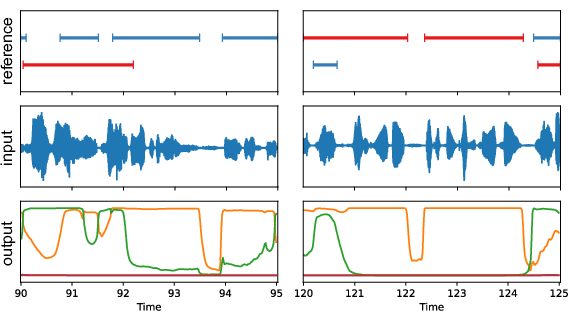
\includegraphics[width=\textwidth,height=0.8\textheight,keepaspectratio]{images/audio-nlp/pyannote_output.png}
    \end{center}
    \vspace{-0.4em}
    {\scriptsize Reference annotation (top) against the model's frame-wise speaker posteriors (bottom). Source: \texttt{pyannote.audio}.}
\end{frame}

\begin{frame}[allowframebreaks]{Emotion Recognition}
    \begin{itemize}
        \item \textbf{Goal:} Detect emotions from speech signals
        \item \textbf{Applications:}
            \begin{itemize}
                \item Human-computer interaction
                \item Mental health monitoring
                \item Customer service analytics
            \end{itemize}
        \item \textbf{Datasets:} IEMOCAP, RAVDESS, MSP-IMPROV, CREMA-D
    \end{itemize}
    \begin{center}
        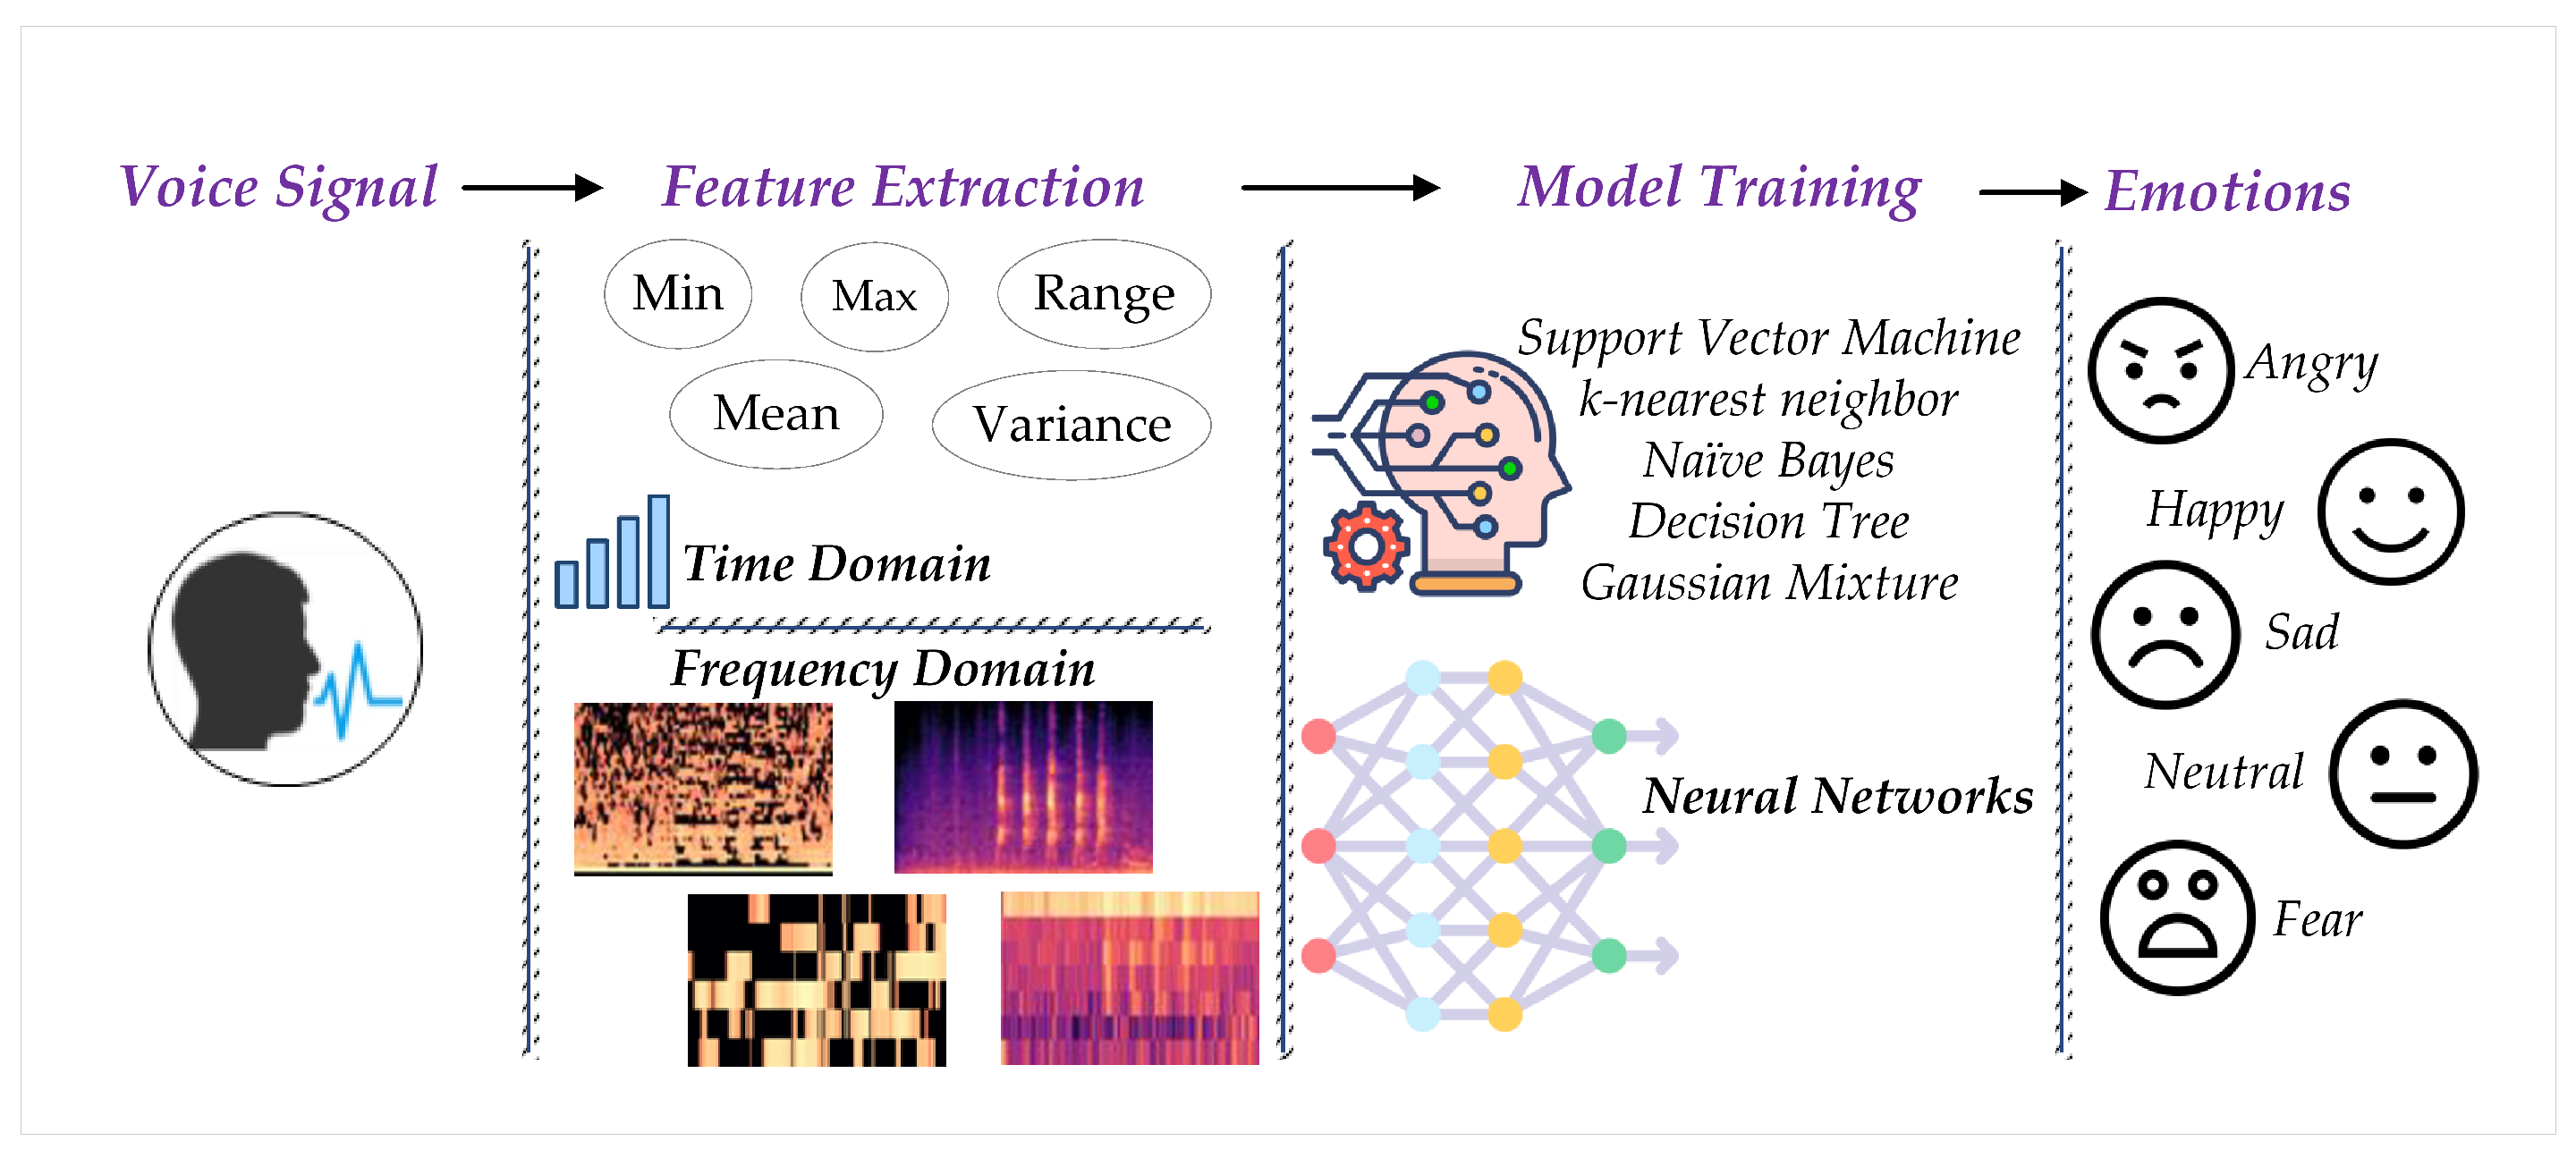
\includegraphics[width=\textwidth,height=0.7\textheight,keepaspectratio]{images/audio-nlp/emotion_classes.png}\\
        {\scriptsize The classical SER pipeline. Source: A.~S.~Alluhaidan, O.~Saidani, R.~Jahangir, M.~A.~Nauman and O.~S.~Neffati, ``Speech Emotion Recognition through Hybrid Features and Convolutional Neural Network,'' \emph{Applied Sciences} 13(8):4750, 2023, Fig.~1 (CC BY 4.0).}
    \end{center}
\end{frame}

\begin{frame}[allowframebreaks]{Emotion Recognition: Models}
    \begin{itemize}
        \item The standard recipe is a \textbf{self-supervised speech encoder plus a light classifier head}:
            \begin{itemize}
                \item \textbf{Wav2Vec 2.0}, \textbf{HuBERT}, \textbf{WavLM}: general-purpose encoders, robust to noise and speaker variation
                \item \textbf{emotion2vec}: pre-trained on emotion data specifically
                \item Frames are pooled (mean or attention pooling) and passed to a small classifier
            \end{itemize}
        \item \textbf{Performance on IEMOCAP} (4-class: angry, happy, neutral, sad):
            \begin{itemize}
                \item $\sim$63--68\% accuracy with the encoder \emph{frozen} and only a linear head trained
                \item $\sim$73--75\% once the encoder itself is \emph{fine-tuned}
            \end{itemize}
        \item \textbf{Compare numbers with care.} IEMOCAP results are almost always reported on the 4-class collapse with ``excited'' merged into ``happy'', under leave-one-session-out splits, and papers differ on whether they quote weighted (WA) or unweighted (UA) accuracy. Two figures from different papers are usually not comparable.
    \end{itemize}
\end{frame}

\begin{frame}{Visual Speech Recognition: Lipreading (LipNet)}
    \begin{itemize}
        \item \textbf{LipNet} (Assael et al., 2016) decodes sentences from lip movement alone, with no audio at all.
        \item \textbf{Architecture:} spatiotemporal convolutions over the video frames $\rightarrow$ bidirectional GRU $\rightarrow$ CTC loss, trained end to end. The same CTC machinery as in audio ASR, with video frames in place of spectrogram frames.
        \item \textbf{Result:} 95.2\% sentence-level accuracy on the GRID corpus (overlapped-speaker split), against 86.4\% for the previous word-level state of the art.
        \item \textbf{Why it matters:} it gives a channel that survives when the audio does not. Fusing the two, \emph{audio-visual} speech recognition, improves accuracy in noise.
    \end{itemize}
    \begin{center}
        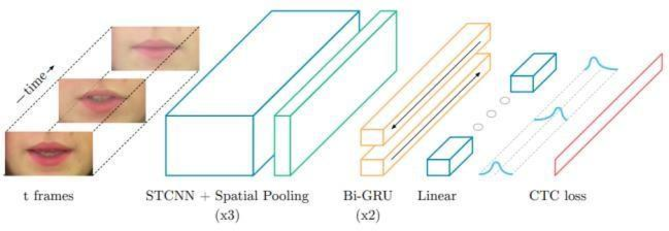
\includegraphics[width=0.82\textwidth,height=0.22\textheight,keepaspectratio]{images/audio-nlp/lipnet_architecture.png}\\
        {\scriptsize Source: Assael et al., ``LipNet: End-to-End Sentence-level Lipreading'', 2016, Fig.~1.}
    \end{center}
\end{frame}
